\documentclass[12pt,aspectratio=1610]{beamer}
\RequirePackage{
    amsmath,
    amssymb,
    calc,
    cancel,
    booktabs,
    color,
    siunitx,
    tikz,
    wrapfig,
    array,
    leftidx,
    float,
    etoolbox,
    fancyhdr,
    longtable,
    hyperref,
    ltcaption,
    ulem,
    wasysym,
    accents,
    listings,
    tabularx,
}

\hypersetup{
    hidelinks,
    breaklinks              = true,
}

\usepackage[final]{pdfpages}
\usepackage[many]{tcolorbox}

\RenewDocumentCommand{\vec}{m}{\mathbf{#1}}

\makeatletter
    \def\new@mathgroup{\alloc@8\mathgroup\mathchardef\@cclvi}
    \patchcmd{\document@select@group}{\sixt@@n}{\@cclvi}{}{}
    \patchcmd{\select@group}{\sixt@@n}{\@cclvi}{}{}
\makeatother

\RequirePackage{mathspec}                                   % includes fontspec
\RequirePackage{polyglossia}                                % multi-language support
\RequirePackage{xunicode}
\setdefaultlanguage{slovak}

% Setup fonts -- see fontspec/mathspec documentation.
\defaultfontfeatures{
    Mapping         = tex-text,
    Scale           = MatchLowercase,
    Ligatures       = TeX
}


\NewDocumentCommand{\labelmath}{m +m}{%
    \begin{equation}%
        #2%
        \label{#1}%
    \end{equation}%
}

\NewDocumentCommand{\labelalign}{m +m}{%
    \begin{align}%
        #2%
        \label{#1}%
    \end{align}%
}

\linespread{1.0}
\setlength{\parindent}{0cm}
\setlength{\parskip}{6pt}
\setlength{\abovedisplayskip}{0mm}
\setlength{\belowdisplayskip}{0mm}
\setlength{\abovedisplayshortskip}{0mm}
\setlength{\belowdisplayshortskip}{0mm}
\setlength{\itemindent}{0pt}
\setlength{\textfloatsep}{0mm}
\setlength{\tabcolsep}{3mm}
\setlength{\LTcapwidth}{0.8\textwidth}
\renewcommand{\arraystretch}{1.2}

\setcounter{secnumdepth}{2}

/home/kvik/dgs/core/tex/math.tex
\DeclareSIUnit\au{AU}
\DeclareSIUnit\pixel{px}
\DeclareSIUnit\lightyear{ly}
\DeclareSIUnit\parsec{pc}
\DeclareSIUnit\earthmass{M_{\earth}}
\DeclareSIUnit\speedoflight{c}
\DeclareSIUnit\foe{foe}
\DeclareSIUnit\year{yr}
\DeclareSIUnit\eur{€}
\DeclareSIUnit\solarmass{M_{\astrosun}}
\DeclareSIUnit\solarluminosity{L_{\astrosun}}
\DeclareSIUnit{\byte}{B}




\linespread{1.0}
\setlength{\parindent}{0cm}
\setlength{\parskip}{6pt}
\setlength{\abovedisplayskip}{0mm}
\setlength{\belowdisplayskip}{0mm}
\setlength{\abovedisplayshortskip}{0mm}
\setlength{\belowdisplayshortskip}{0mm}
\setlength{\itemindent}{0pt}
\setlength{\textfloatsep}{0mm}
\setlength{\tabcolsep}{3mm}
\renewcommand{\arraystretch}{1.2}

\setcounter{secnumdepth}{0}

\NewDocumentCommand{\fspicture}{m O{W} O{black}}{
    {
        \setbeamertemplate{navigation symbols}{}
        \setbeamercolor{background canvas}{bg = #3}
        \begin{frame}[plain]
            \begin{tikzpicture}[remember picture, overlay]
                \node[at=(current page.center)] {
                    \ifstrequal{H}{#2}{                                  
                        \includegraphics[height=\paperheight]{#1}%
                    }{%
                        \includegraphics[width=\paperwidth]{#1}%
                    }
                };
            \end{tikzpicture}
        \end{frame}
    }
}

\NewDocumentCommand{\frejm}{m +m}{
    \begin{frame}
        \frametitle{#1}
        #2
    \end{frame}
}

\NewDocumentCommand{\fragfrejm}{m +m}{
    \begin{frame}[fragile]
        \frametitle{#1}
        #2
    \end{frame}
}

\defbeamertemplate{description item}{align center}{\hfill\insertdescriptionitem\hfill}
\definecolor{desc}{rgb}{0.66, 0, 0}
\definecolor{citem}{rgb}{0.72, 0, 0}
\definecolor{csitem}{rgb}{0.90, 0, 0}
\definecolor{cssitem}{rgb}{1, 0.1, 0.1}
\definecolor{qprimarybg}{rgb}{0.95, 0.95, 0.95}
\definecolor{check}{rgb}{0, 0.8, 0}
\definecolor{coded}{rgb}{0.9, 0.9, 0.9}
\definecolor{todo}{rgb}{1.0, 0.3, 0.3}
\definecolor{model}{rgb}{0.75, 0, 0}

\setbeamertemplate{navigation symbols}{}
\newfontfamily{\semibold}{Segoe UI Semibold}
\RenewDocumentCommand{\emph}{m}{{\semibold#1}}
\NewDocumentCommand{\code}{m}{\textcolor{desc}{\texttt{#1}}}
\NewDocumentCommand{\model}{m}{\colorbox{coded}{\textcolor{model}{\texttt{#1}}}}
\NewDocumentCommand{\todo}{m}{\colorbox{todo}{#1}}

\mode<presentation> {
    \usetheme{Szeged}
    \usecolortheme{beaver}
    
    \usefonttheme{professionalfonts}
    \setallmainfonts{Minion Pro}
    \setmathrm{Minion Pro}
    
    \setsansfont{Segoe UI}
    \setmonofont{Consolas}
    \setbeamercolor*{enumerate item}{fg = citem}
    \setbeamercolor*{enumerate subitem}{fg = csitem}
    \setbeamercolor*{enumerate subsubitem}{fg = cssitem}
    \setbeamercolor*{description item}{fg = desc}
    \setbeamercolor*{itemize item}{fg = citem}
    \setbeamercolor*{itemize subitem}{fg = csitem}
    \setbeamercolor*{itemize subsubitem}{fg = cssitem}
    \setbeamercolor*{palette primary}{fg = red, bg = qprimarybg}
}

\newcommand<>\highlightbox[2]{%
    \alt#3{\makebox[\dimexpr\width-2\fboxsep]{\colorbox{#1}{#2}}}{#2}%
}

\AtBeginSection[]{
    \subsection{\insertsection}
    \begin{frame}
        \vfill
        \centering
        \begin{beamercolorbox}[sep = 18pt, center, shadow = true, rounded = true]{title}
            \usebeamerfont{title}\insertsectionhead%
            \vfill
        \end{beamercolorbox}
        \vfill
    \end{frame}
}

\makeatletter
% Render percent sign with nice font, not ugly Computer modern
    \mathcode`\%="7025

% Fixes mathspec bug -- URL numbers are rendered with wrong font
    \ernewcommand\eu@MathPunctuation@symfont{Latin:m:n}
    \DeclareMathSymbol{,}{\mathpunct}{\eu@MathPunctuation@symfont}{`,}
    \DeclareMathSymbol{?}{\mathpunct}{\eu@MathPunctuation@symfont}{`?}
    \DeclareMathSymbol{.}{\mathord}{\eu@MathPunctuation@symfont}{`.}
    \DeclareMathSymbol{<}{\mathrel}{\eu@MathPunctuation@symfont}{`<}
    \DeclareMathSymbol{>}{\mathrel}{\eu@MathPunctuation@symfont}{`>}
    \DeclareMathSymbol{/}{\mathord}{\eu@MathPunctuation@symfont}{`/}
    \DeclareMathSymbol{;}{\mathpunct}{\eu@MathPunctuation@symfont}{`;}
    \DeclareMathSymbol{(}{\mathopen}{\eu@DigitsArabic@symfont}{`(}
    \DeclareMathSymbol{)}{\mathclose}{\eu@DigitsArabic@symfont}{`)}
    \XeTeXDeclareMathSymbol{^^^^2026}{\mathinner}{\eu@MathPunctuation@symfont}{"2026}[\mathellipsis]
    \DeclareMathSymbol{0}{\mathalpha}{\eu@DigitsArabic@symfont}{`0}
    \DeclareMathSymbol{1}{\mathalpha}{\eu@DigitsArabic@symfont}{`1}
    \DeclareMathSymbol{2}{\mathalpha}{\eu@DigitsArabic@symfont}{`2}
    \DeclareMathSymbol{3}{\mathalpha}{\eu@DigitsArabic@symfont}{`3}
    \DeclareMathSymbol{4}{\mathalpha}{\eu@DigitsArabic@symfont}{`4}
    \DeclareMathSymbol{5}{\mathalpha}{\eu@DigitsArabic@symfont}{`5}
    \DeclareMathSymbol{6}{\mathalpha}{\eu@DigitsArabic@symfont}{`6}
    \DeclareMathSymbol{7}{\mathalpha}{\eu@DigitsArabic@symfont}{`7}
    \DeclareMathSymbol{8}{\mathalpha}{\eu@DigitsArabic@symfont}{`8}
    \DeclareMathSymbol{9}{\mathalpha}{\eu@DigitsArabic@symfont}{`9}
\makeatother


\title{AMOS data processing pipeline}
\subtitle{Writing astronomical software, one mistake at a time}
\author{\small \emph{Martin Baláž}}
\institute{DAA colloquium}
\date{2021--02--17}

\begin{document}
    {
%        \usebackgroundtemplate{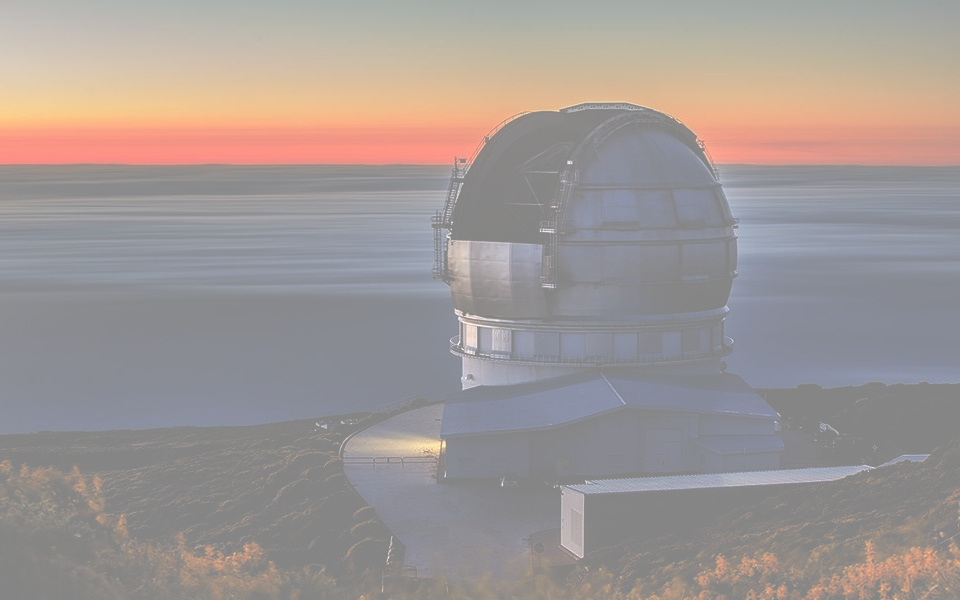
\includegraphics[width=\paperwidth]{pictures/gtc.jpg}}
        \begin{frame}
            \titlepage
        \end{frame}
    }

    \section{Overview}
        \frejm{Contents}{
            \setbeamersize{description width = 30mm}
            \begin{description}
                \item[objective]        What are we doing?
                \item[motivation]       Why?
                \item[implementation]   How?
                \item[results]          What have we done?
            \end{description}
        }

        \frejm{AMOS}{
            \emph{A}ll-sky \emph{M}eteor \emph{O}rbit \emph{S}ystem
            \begin{columns}
                \begin{column}{0.6\textwidth}
                    \begin{itemize}
                        \item a network of 11 all-sky cameras
                        \item permanent surveillance of the skies
                        \item trilateration of meteor trajectories
                    \end{itemize}
                \end{column}
                \begin{column}{0.39\textwidth}
                    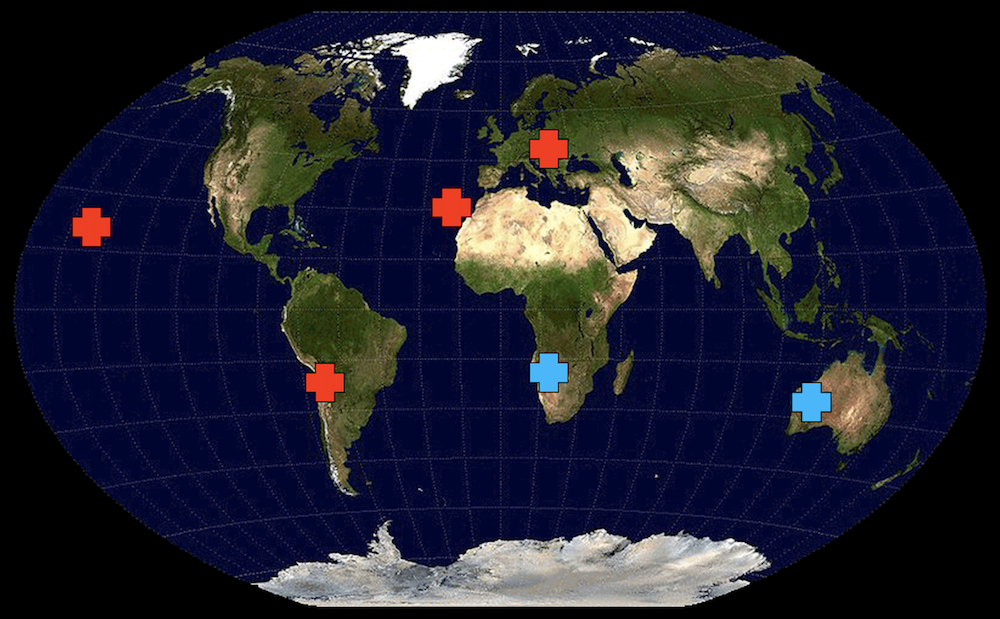
\includegraphics[width=\linewidth]{pictures/amos-map.png}
                \end{column}
            \end{columns}
        }

        \fspicture{pictures/amos-view.jpg}[H][black]

        \frejm{Objective and motivation}{
            Current state is \only<1>{a disaster}\only<2->{\sout{a disaster} slightly suboptimal}
            \pause
            \begin{itemize}
                \item no unified data file format
                \item data spread across multiple computers
                \item analysis very difficult
            \end{itemize}
            \pause
            \emph{Let us tidy up and organize the data!}
        }

        \frejm{Illustration}{
            \begin{columns}
                \begin{column}{0.46 \textwidth}
                    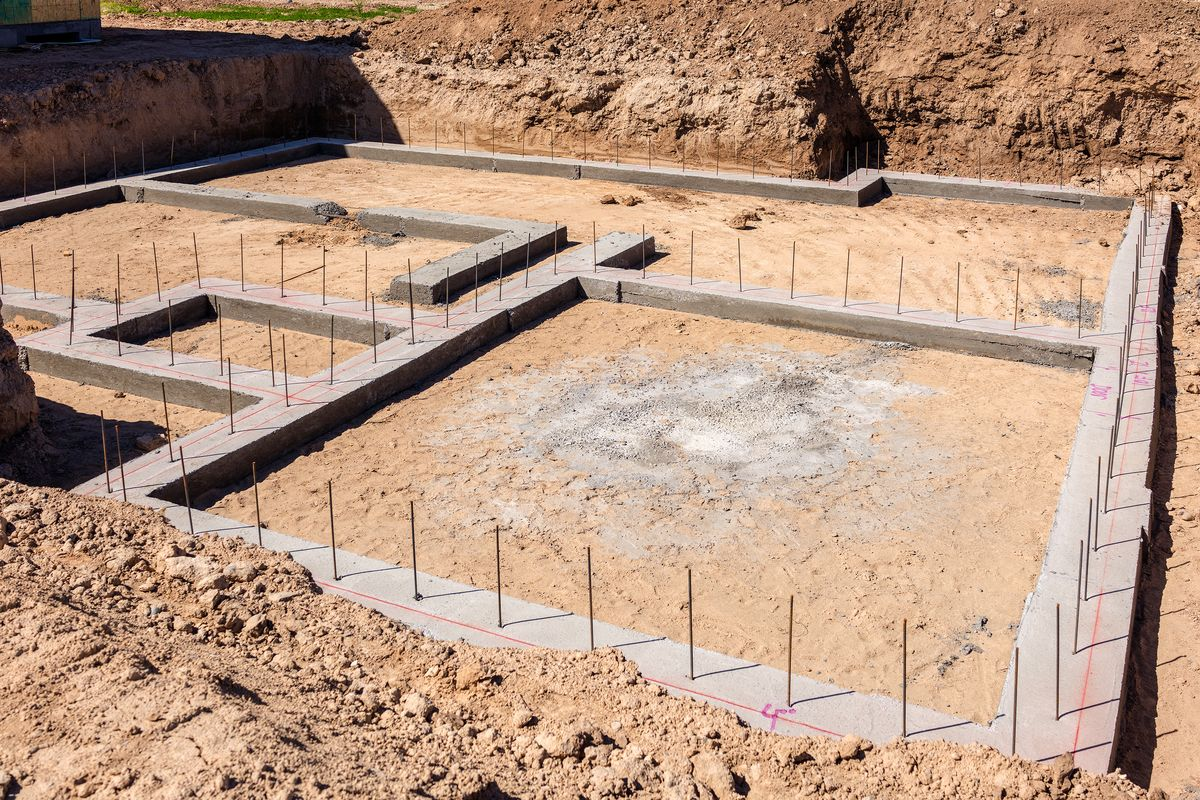
\includegraphics[width=\linewidth]{pictures/foundations.jpg}
                \end{column}
                \pause
                \begin{column}{0.05 \textwidth}
                    $\Rightarrow$
                \end{column}
                \begin{column}{0.46 \textwidth}
                    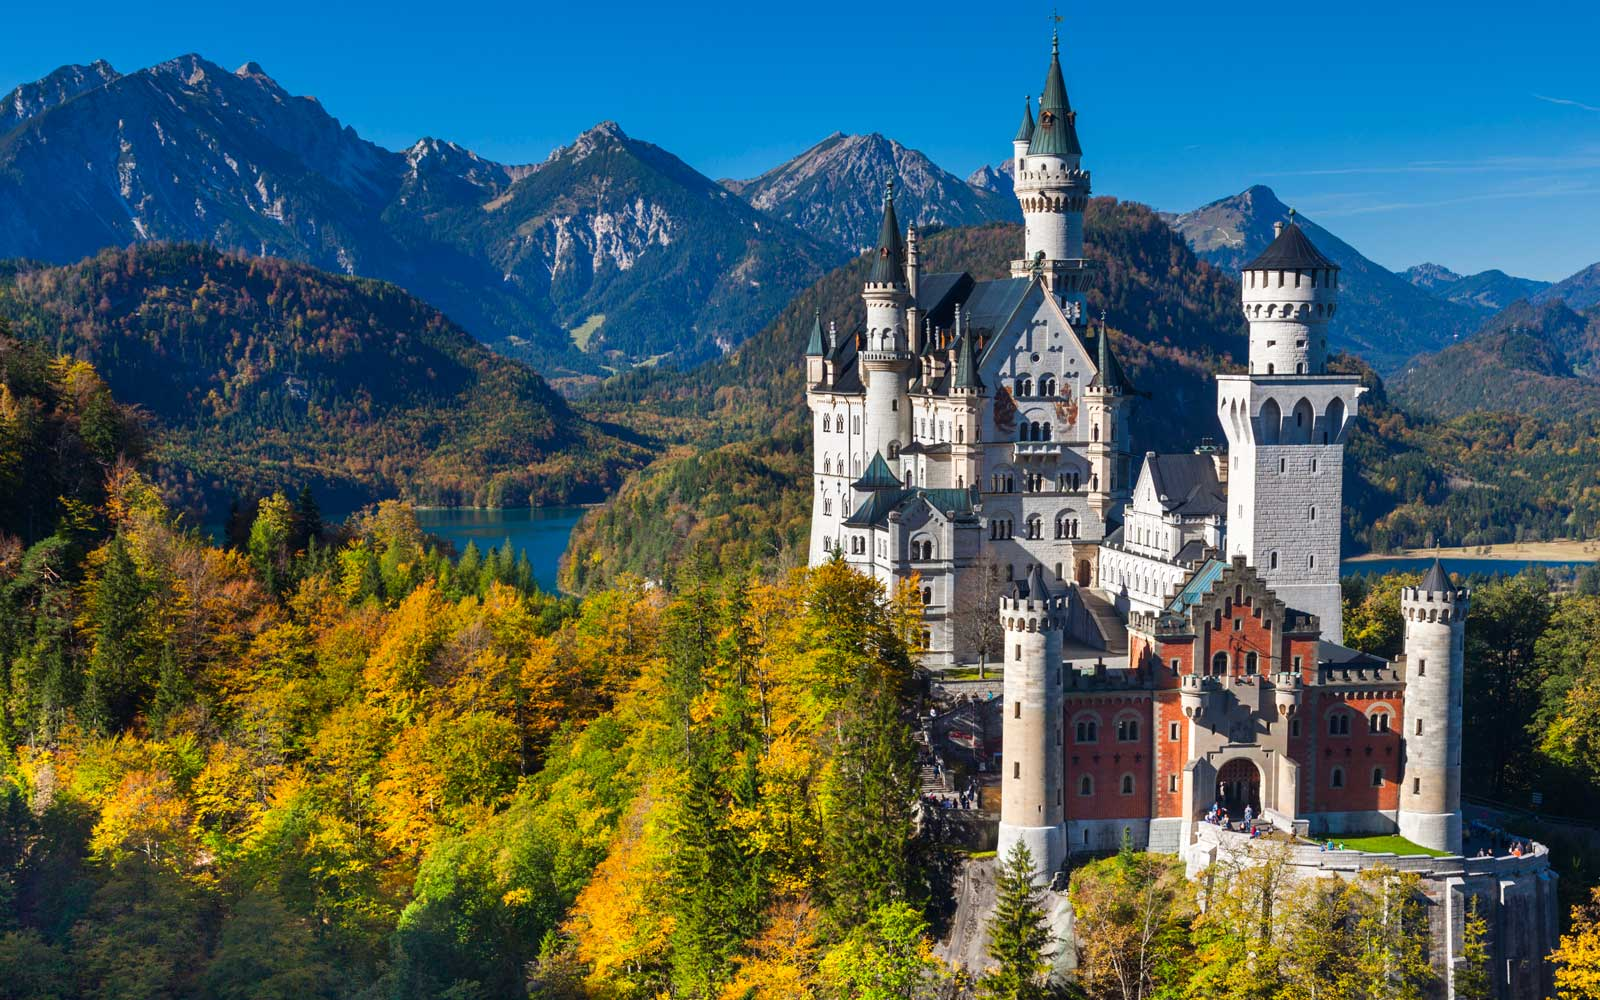
\includegraphics[width=\linewidth]{pictures/neuschwanstein.jpg}
                \end{column}
            \end{columns}
        }

        \frejm{Pipeline}{
            \begin{itemize}
                \item data acquisition
                    \begin{itemize}
                        \item 11 stations in various stages of decay
                        \item dome with all-sky camera
                        \item computer with software
                        \pause
                        \item \textcolor{gray}{optionally spectral camera}
                    \end{itemize}
                \pause
                \item preprocessing
                    \begin{itemize}
                        \item image recognition
                    \end{itemize}
                \item retrieval and storage
                \item trajectory and orbit computation
                \item storage of final data
            \end{itemize}
        }

        \frejm{Plan}{
            \begin{columns}
                \begin{column}{0.49\textwidth}
                    Replace the \emph{old stack}...
                    \begin{itemize}
                        \item \code{daemon.exe} (daemon)
                        \item \code{client.exe} (console)
                        \item \code{launcher.exe} (service)
                        \item \code{cleaner.exe} (service)
                        \item Synology (network drive)
                        \item mystery script on \code{charon} (???)
                        \item folder listing
                    \end{itemize}
                \end{column}
                \pause
                \begin{column}{0.49\textwidth}
                    ...by the \emph{new stack}!
                    \begin{itemize}
                        \item \code{AMOS controller} (GUI application)
                            \begin{itemize}
                                \item controls the dome
                                \item manages \code{UFO}, local storage
                            \end{itemize}
                        \item \code{AMOS server}
                            \begin{itemize}
                                \item persistent storage
                                \item bindings to \code{MT}
                                \item data analysis
                            \end{itemize}
                    \end{itemize}
                \end{column}
            \end{columns}
        }

        \fspdfpage{pictures/full.pdf}{1}[H][white]

    \section{Client side}
        \frejm{Remote station}{
            \begin{columns}
                \begin{column}{0.49\textwidth}
                    Various components as available
                    \begin{itemize}
                        \item mini-ITX motherboard
                        \item dome control
                            \begin{itemize}
                                \item electronics by Pavol Zigo
                            \end{itemize}
                        \item Synology (network drive)
                        \item own router
                            \begin{itemize}
                                \item source of problems
                            \end{itemize}
                    \end{itemize}
                \end{column}
                \pause
                \begin{column}{0.49\textwidth}
                    Unified design
                    \begin{itemize}
                        \item new mini-ITX motherboard
                            \begin{itemize}
                                \item ideally does not burn
                            \end{itemize}
                        \item same dome control
                        \item 2× 4 TB HDD in \code{RAID1}
                        \item no network drive
                        \item no router
                        \item metadata on server
                    \end{itemize}
                \end{column}
            \end{columns}

        }

        \fspicture{pictures/amos-pc.jpg}

        \fspicture{pictures/amos-inside.jpg}

        \frejm{Pre-processing}{
            First of all, raw data are filtered and annotated

            \begin{itemize}
                \item meteor recognition and data extraction
                \begin{itemize}
                    \item position in the sky
                    \item magnitude
                    \item angular speed
                    \item ...
                \end{itemize}
                \pause
                \item saved in an \code{XML} file
                \item raw video stored in an uncompressed \code{AVI} file
                \item overview in a \code{JPG} file
            \end{itemize}
            \pause
            \begin{itemize}
                \item \code{UFO} ...not much can be easily done about this
            \end{itemize}
        }

        \frejm{UFOCaptureV2}{
            \begin{itemize}
                \item problems with video codec \code{Y16} vs \code{Y800}
                \item mysterious flashes (maybe II?)
                \item old, weakly supported
                \pause
                \item basically a \emph{black box}
                \item complex configuration
                \pause
                \item we should move to the \emph{Kvant} software
                \begin{itemize}
                    \item problem with frame rate
                \end{itemize}
            \end{itemize}
        }

        \frejm{Technology}{
            We want a \emph{GUI} application (Windows 10)... \emph{AMOS client / controller}
            \pause

            After a lengthy decision process... \emph{C++} and \emph{Qt5}
            \begin{columns}
                \begin{column}{0.75\textwidth}
                    \begin{itemize}
                        \item multi-platform
                        \item \emph{great} documentation
                        \item free (under \emph{GPL})
                        \item Python bindings also available (PyQt)
                    \end{itemize}
                \end{column}
                \begin{column}{0.15\textwidth}
                    
\includegraphics[width=\linewidth]{pictures/qt.png}
                    \\[5mm]
                    
\includegraphics[width=\linewidth]{pictures/c++.png}
                \end{column}
            \end{columns}
        }

        \frejm{Implementation}{
            \begin{itemize}
                \item Montenbruck C++ astronomy library
                \item logic from old \code{daemon.exe}
                \pause
                \item lots of improvements
                    \begin{itemize}
                        \item full display of status
                        \item manual control
                        \item visible to the user
                        \item notifications
                    \end{itemize}
            \end{itemize}
        }

        \frejm{Retrieval}{
            \begin{columns}
                \begin{column}{0.49\textwidth}
                    \emph{Old}:
                    \begin{itemize}
                        \item UFOCapture launches a \code{bat} file
                        \item mail transfer via SMTP (e-mail)
                        \item processed by \code{charon}
                    \end{itemize}
                \end{column}
                \pause
                \begin{column}{0.49\textwidth}
                    \emph{New}:
                    \begin{itemize}
                        \item client scans the output directory
                        \item files moved to correct subdirectory
                            \begin{itemize}
                                \item \code{yyyy/mm/dd}
                            \end{itemize}
                        \item sent over HTTP in a POST request
                            \begin{itemize}
                                \item \code{JPG}, \code{XML}, \code{AVI} size
                            \end{itemize}
                    \end{itemize}
                \end{column}
            \end{columns}
        }

    \section{Server side}
        \frejm{Design criteria}{
            \begin{itemize}
                \item has a \emph{public IP}
                \begin{itemize}
                    \item clients do not (VPN, NAT, Chilean desert)
                    \item server is always available
                \end{itemize}
                \item contains all final data
            \end{itemize}
        }


        \frejm{Storage}{
            How to store all the data?
            \pause
            \begin{itemize}
                \item in a \emph{structured} and \emph{semantic} way
                \item consistency \emph{enforced} at all times
                \item also auxiliary data
                \begin{itemize}
                    \item housekeeping
                    \item statistics
                    \item user accounts...
                \end{itemize}
            \end{itemize}
        }

        \frejm{Data retention}{
            To prevent problems down the line, we should
            \pause
            \begin{itemize}
                \item \emph{never} delete anything
                \begin{itemize}
                    \item unless provably \emph{incorrect}
                \end{itemize}
                \pause
                \item enable raw data re-processing
                \begin{itemize}
                    \item data import from an offline station
                    \item manual correction
                    \item new processing algorithms
                \end{itemize}
            \end{itemize}
        }

        \frejm{Housekeeping}{
            \textit{Def:} Data of little or \emph{no scientific value} but \emph{high operational importance} \\[10mm]
            \pause
            \begin{columns}
                \begin{column}{0.33\textwidth}
                    \begin{itemize}
                        \item environment
                            \begin{itemize}
                                \item rain
                                \item temperature
                                \item humidity
                                \item ...
                            \end{itemize}
                    \end{itemize}
                \end{column}
                \begin{column}{0.33\textwidth}
                    \begin{itemize}
                        \item station
                            \begin{itemize}
                                \item cover status
                                \item system uptime
                                \item disk usage
                                \item ...
                            \end{itemize}
                    \end{itemize}
                \end{column}
                \begin{column}{0.33\textwidth}
                    \begin{itemize}
                        \item network
                            \begin{itemize}
                                \item connection
                                \item last data
                                \item ...
                            \end{itemize}
                    \end{itemize}
                \end{column}
            \end{columns}
            \pause
            \vspace{8mm}
            \begin{itemize}
                \item sent as \model{Heartbeat}
                \item everything displayed in a \emph{dashboard}
            \end{itemize}
        }

    \section{Database}
        \frejm{The database}{
            \emph{Problem}: We need a way to visualize and comprehend the data

            \pause
            \emph{Solution}: A database and a web interface
            \begin{itemize}
                \item provides a basic framework for data operations
                \item more user-friendly than bare directory listing
                \item easier to retrieve, sort and analyze the data
            \end{itemize}
        }

        \frejm{Design}{
            Underlying data are well-structured and suitable for an \emph{object-relational} database

            \begin{itemize}
                \item data are stored in \emph{relations} (tables)
                \item each column stores the same \emph{property}
                \item each row stores a single \emph{entity} (object)
                \item each object has an identifier -- \emph{primary key}
                \item fields may point to other tables -- \emph{foreign keys}
                \item data are accessed and manipulated using a \emph{query language}
            \end{itemize}
        }

        \begin{frame}[fragile]
            \frametitle{SQL example}
            \small
            \begin{overlayarea}{\textwidth}{0.7 \textheight}
                \ \\
                \highlightbox<2>{orange}{\texttt{SELECT "id", "timestamp", "magnitude" \textbackslash}} \\
                \highlightbox<3>{orange}{\texttt{FROM "meteors" \textbackslash}} \\
                \highlightbox<4>{orange}{\texttt{WHERE "timestamp" BETWEEN "2021-02-16 18:00:00" AND "2021-02-17 06:00:00" \textbackslash}} \\
                \highlightbox<5>{orange}{\texttt{ORDER BY "magnitude" ASC \textbackslash}} \\
                \highlightbox<6>{orange}{\texttt{LIMIT 5;}}
                \vspace{5mm}

                \begin{onlyenv}<7>
                    Response:
                \begin{verbatim}
356, "2021-04-17 03:45:10", -5.8
728, "2021-04-17 04:14:23", -3.2
456, "2021-04-16 23:56:04", -2.7
908, "2021-04-17 01:23:45", -2.5
854, "2021-04-16 21:58:35", -2.2
                \end{verbatim}
                \end{onlyenv}
            \end{overlayarea}
        \end{frame}

        \frejm{Models}{
            The art and science of creating databases...

            \pause
            ...is in how to naturally translate the real world to models:
            \pause
            \begin{itemize}
                \item \model{Meteor}
                \item \model{Sighting}
                \item \model{Station}
                \item \model{Subnetwork}
                \item \model{Country}
                \item ...more as needed
            \end{itemize}
        }

        \fspdfpage{pictures/schema.pdf}{2}[W][white]

    \section{Visualisation}
        \frejm{Overview}{
            We have implemented a website in \emph{Python/Django}

            \begin{itemize}
                \item webserver + CRUD operations
                \item administration interface (courtesy of Django)
                \item REST framework
            \end{itemize}
        }

        \frejm{Dashboard}{
            We need to detect problems and bring them to attention
            \pause
            \begin{itemize}
                \item various problems can be detected and addressed
                \begin{itemize}
                    \item lost connection
                    \item lost power
                    \item software problems
                    \item AMOS hardware failure
                    \item no data
                    \item ...
                \end{itemize}
            \end{itemize}
        }

    \section{Summary}
        \frejm{And then?}{
            The system enables us to do much more:
            \begin{columns}
                \begin{column}{0.6\textwidth}
                    \begin{itemize}
                        \item sort and display meteors by any criteria
                        \pause
                        \item display meteor activity
                        \item use data from \code{Asmodeus} to estimate flux
                        \pause
                        \item provide foundation for my PhD thesis
                        \pause
                        \item data for \emph{you}
                    \end{itemize}
                \end{column}
                \begin{column}{0.3\textwidth}
                    
\includegraphics[width = \linewidth]{pictures/unclesam.jpg}
                \end{column}
            \end{columns}
        }

        \frejm{Thank you for your attention}{
            {\large \textit{Above all else, show the data.}}
            \scriptsize
            \begin{flushright}
                Edward R. Tufte\\
                The Visual Display of Quantitative Information, 1983
            \end{flushright}
        }

        \frejm{References}{
            \begin{itemize}
                \item \textbf{Database.Guide}:
                    What is an ORDBMS? \texttt{https://database.guide/what-is-an-ordbms/}
                \item \textbf{James Montgomery Flagg}:
                    Uncle Sam Needs You (US Propaganda material). 1917.
                \item \textbf{holistics.io}:
                    \texttt{dbdiagram.io} database relationship diagram tool. \texttt{https://dbdiagram.io/}.
            \end{itemize}
        }




\end{document}
